\begin{block}{Introducing Randomness}

	\begin{figure}
		\centering
		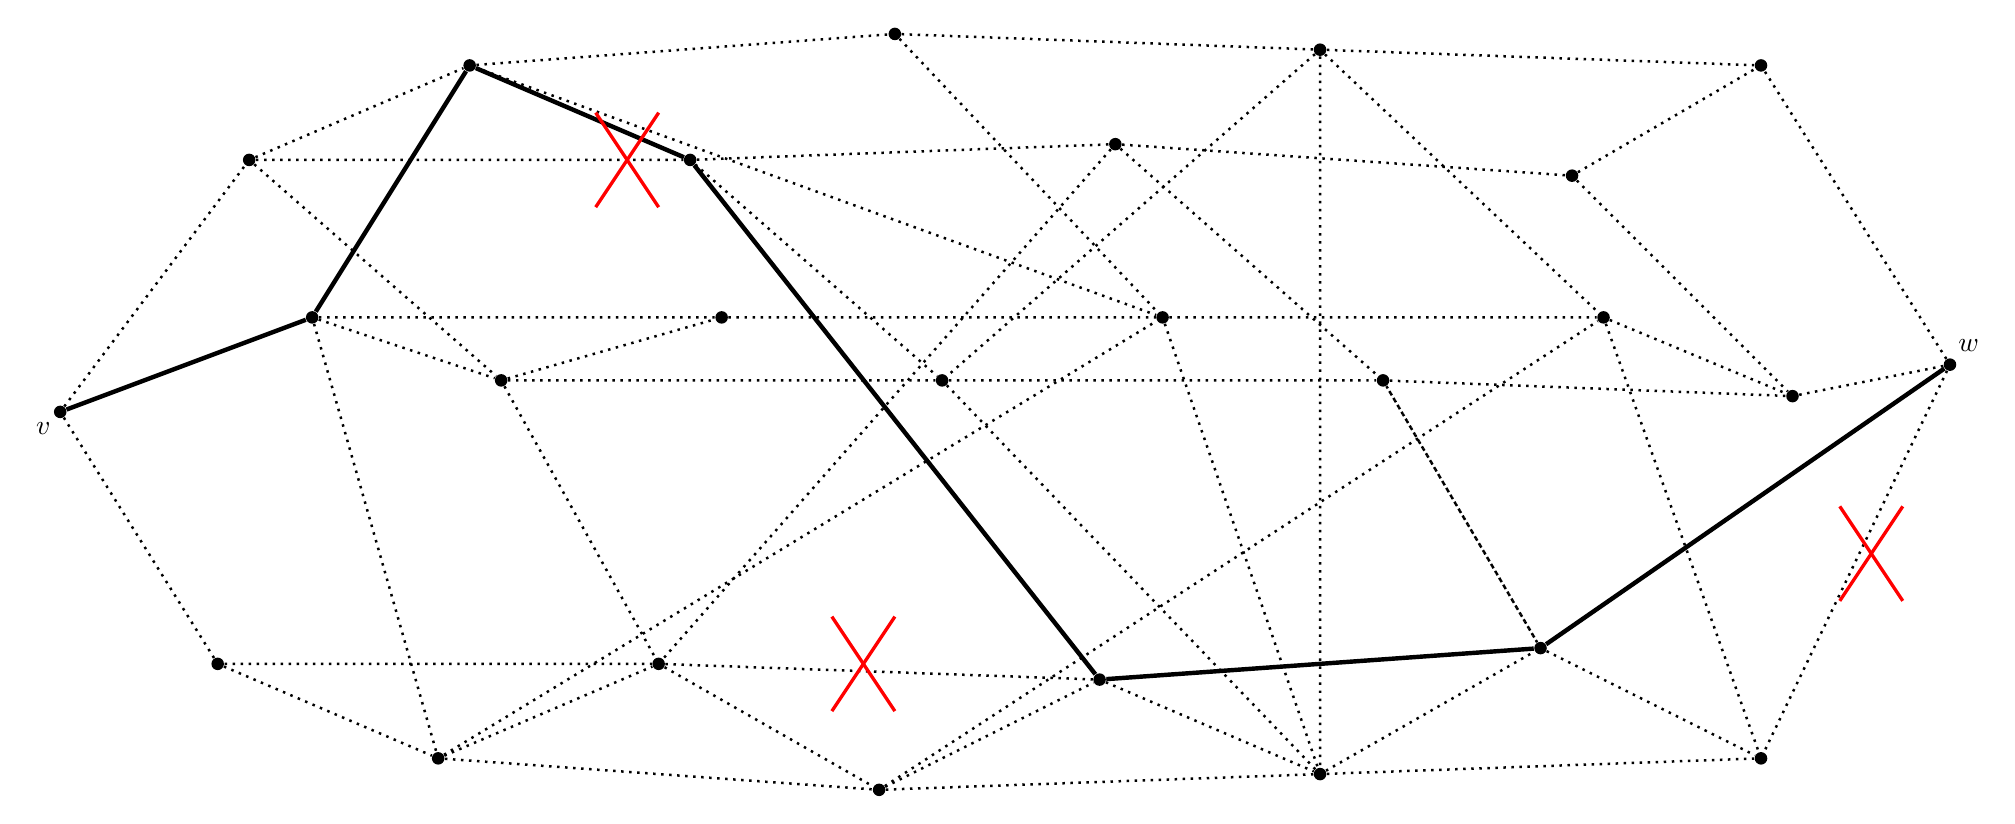
\begin{tikzpicture}[
			scale=2.0,
			every node/.style={circle, fill=black, inner sep=1.6pt},
			bg/.style={draw, ellipse, very thick},
			noise/.style={dotted, line width=0.9pt},
			path/.style={ultra thick},
			]


			% --- Nodes (lots of them) ---
			\node (v) at (0,0) {};
			\node (w) at (12,0.3) {};

			\node (a1) at (1.2,1.6) {}; \node (a2) at (2.6,2.2) {}; \node (a3) at (4.0,1.6) {};
			\node (a4) at (5.3,2.4) {}; \node (a5) at (6.7,1.7) {}; \node (a6) at (8.0,2.3) {};
			\node (a7) at (9.6,1.5) {}; \node (a8) at (10.8,2.2) {};

			\node (b1) at (1.6,0.6) {}; \node (b2) at (2.8,0.2) {}; \node (b3) at (4.2,0.6) {};
			\node (b4) at (5.6,0.2) {}; \node (b5) at (7.0,0.6) {}; \node (b6) at (8.4,0.2) {};
			\node (b7) at (9.8,0.6) {}; \node (b8) at (11.0,0.1) {};

			\node (c1) at (1.0,-1.6) {}; \node (c2) at (2.4,-2.2) {}; \node (c3) at (3.8,-1.6) {};
			\node (c4) at (5.2,-2.4) {}; \node (c5) at (6.6,-1.7) {}; \node (c6) at (8.0,-2.3) {};
			\node (c7) at (9.4,-1.5) {}; \node (c8) at (10.8,-2.2) {};

			% Labels for endpoints
			\node[fill=none, below left=2pt] at (v) {$v$};
			\node[fill=none, above right=2pt] at (w) {$w$};

			% --- MANY dotted/noise edges (looks dense) ---
			% Top layer connections
			\draw[noise] (a1)--(a2)--(a3) (a7)--(a8);
			\draw[noise] (a1)--(a3) (a2)--(a4) (a3)--(a5) (a4)--(a6) (a5)--(a7) (a6)--(a8);

			% Middle layer connections
			\draw[noise] (b1)--(b2)--(b3) (b7)--(b8);
			\draw[noise] (b1)--(b3) (b2)--(b4) (b3)--(b5) (b4)--(b6) (b5)--(b7) (b6)--(b8);

			% Bottom layer connections
			\draw[noise] (c1)--(c2)--(c3)--(c4)--(c5)--(c6)--(c7)--(c8);
			\draw[noise] (c1)--(c3) (c2)--(c4) (c3)--(c5) (c4)--(c6) (c5)--(c7) (c6)--(c8);

			% Cross edges (adds a "hairball" feel)
			\draw[noise] (a1)--(b2) (a3)--(b4) (a4)--(b5) (a5)--(b6) (a6)--(b7) (a7)--(b8);
			\draw[noise] (b1)--(c2) (b2)--(c3)  (b5)--(c6) (b6)--(c7) (b7)--(c8);

			% Extra random-ish chords
			\draw[noise] (a2)--(b5) (a6)--(b4) ;
			\draw[noise] (c2)--(b5) (c4)--(b7) (c6)--(b4) (c7)--(b6);
			\draw[noise] (a3)--(c5) (a5)--(c3) (a6)--(c6);

			% Connect endpoints into the mess
			\draw[noise] (v)--(a1) (v)--(b1) (v)--(c1);
			\draw[noise] (w)--(a8) (w)--(b8) (w)--(c8);

			% --- ONE highlighted solid path v -> w ---
			% Pick a clean-ish route through the middle
			\draw[path] (v) -- (b1) -- (a2) -- (a3) -- (c5)  -- (c7) -- (w);

			% --- Red X marks on 3 dotted edges ---
			\draw[red, very thick] (3.4,1.9) -- (3.8,1.3);
			\draw[red, very thick] (3.4,1.3) -- (3.8,1.9);

			\draw[red, very thick] (11.3,-1.2) -- (11.7,-0.6);
			\draw[red, very thick] (11.3,-0.6) -- (11.7,-1.2);

			\draw[red, very thick] (4.9,-1.9) -- (5.3,-1.3);
			\draw[red, very thick] (4.9,-1.3) -- (5.3,-1.9);

		\end{tikzpicture}
		\caption{Graph with Skipped Edges}
	\end{figure}


	Deterministically we have seen that this is \textbf{maximally hard}. There is
	no better way to solve this problem than for Alice to send her entire input to
	Bob. However, we might also consider adding randomness, and allowing for error.
	For instance, if there is a path, it is unlikely that any randomly selected
	vertex will fall on it, so we might consider randomly removing some.

\end{block}

\begin{block}{Set Disjointness}

	To find a lower bound for a random algorithm we can no longer rely on
	embedding equality, as random algorithm's for equality can be bounded
	as low as $\Theta(1)$. Thus, we turn to set disjointness.

	\[
		\textsc{DISJ}(x,y)=
		\begin{cases}
			0 & x \cap y \neq \emptyset \\
			1 & x \cap y = \emptyset
		\end{cases}
	\]

	Set Disjointness gives each player some number of elements from a set,
	and asks if the players have any elements in common. If so, the
	protocol outputs 0, and 1 otherwise. Set Disjointness is usefull when
	studying random algorithms since it has been shown that it requires
	\textbf{maximal \emph{random} communication}.

\end{block}

\begin{block}{Disjoint Gadget and Embedding}

	\begin{figure}
		\centering
		\begin{tikzpicture}[y=1cm, x=1cm, scale=2, every node/.append style={scale=1.2}, inner sep=0pt, outer sep=0pt]
			\node[line width=0.0cm,anchor=south west] (text11) at (7.3, 27.3){$v$};
			\path[draw=black,fill=black,line width=0.0cm,shift={(2.5, 3.7)}] (5.5, 23.4) 
				ellipse (0.1cm and 0.1cm);
			\node[line width=0.0cm,anchor=south west] (text14) at (1.0, 24.7){$Alice$};
			\node[line width=0.0cm,anchor=south west] (text22) at (4.8, 24.8){1};
			\node[line width=0.0cm,anchor=south west] (text23) at (6.3, 24.8){2};
			\node[line width=0.0cm,anchor=south west] (text24) at (7.6, 24.8){3};
			\node[line width=0.0cm,anchor=south west] (text25) at (9.4, 24.8){4};
			\node[line width=0.0cm,anchor=south west] (text26) at (10.6, 24.8){5};
			\node[line width=0.0cm,anchor=south west] (text27) at (7.3, 20.3){$w$};
			\node[line width=0.0cm,anchor=south west] (text28) at (1.0, 23){$Bob$};
			\path[draw=black,line width=0.0cm] (5.5, 24.7) -- (6.8, 24.7);
			\path[draw=black,line width=0.0cm] (8.0, 24.7) -- (6.8, 24.7);
			\path[draw=black,line width=0.0cm] (5.5, 24.7) -- (8.0, 27.2) -- (6.8, 24.7);
			\path[draw=black,line width=0.0cm] (8.0, 27.2) -- (8.0, 24.7);
			\path[draw=black,line width=0.0cm] (9.3, 24.7) -- (8.0, 27.2);
			\path[draw=black,line width=0.0cm] (10.5, 24.7) -- (8.0, 27.2);
			\path[draw=black,line width=0.0cm] (5.5, 23.4) -- (8.0, 20.7) -- (6.8, 23.4);
			\path[draw=black,line width=0.0cm] (8.0, 23.4) -- (8.0, 20.7) -- (9.3, 23.4);
			\path[draw=black,line width=0.0cm] (10.5, 23.4) -- (8.0, 20.7);
			\path[draw=black,line width=0.0cm] (6.8, 24.7) -- (6.8, 23.4); % Line connecting 3--3
			\path[draw=black,fill=black,line width=0.0cm] (5.5, 24.7) ellipse (0.1cm and 
				0.1cm);
			\path[draw=black,fill=black,line width=0.0cm,shift={(1.3, -0.0)}] (5.5, 24.7) 
				ellipse (0.1cm and 0.1cm);
			\path[draw=black,fill=black,line width=0.0cm,shift={(2.5, -0.0)}] (5.5, 24.7) 
				ellipse (0.1cm and 0.1cm);
			\path[draw=black,line width=0.0cm] (9.3, 24.7) -- (8.0, 24.7);
			\path[draw=black,fill=black,line width=0.0cm,shift={(3.8, -0.0)}] (5.5, 24.7) 
				ellipse (0.1cm and 0.1cm);
			\path[draw=black,line width=0.0cm] (10.5, 24.7) -- (9.2, 24.7);
			\path[draw=black,fill=black,line width=0.0cm,shift={(5.0, -0.0)}] (5.5, 24.7) 
				ellipse (0.1cm and 0.1cm);
			\node[line width=0.0cm,anchor=south west] (text22-8) at (4.8, 23.5){1};
			\node[line width=0.0cm,anchor=south west] (text23-4) at (6.3, 23.5){2};
			\node[line width=0.0cm,anchor=south west] (text24-1) at (7.6, 23.5){3};
			\node[line width=0.0cm,anchor=south west] (text25-8) at (9.4, 23.5){4};
			\node[line width=0.0cm,anchor=south west] (text26-8) at (10.6, 23.5){5};
			\path[draw=black,line width=0.0cm] (5.5, 23.4) -- (6.7, 23.4);
			\path[draw=black,line width=0.0cm] (8.0, 23.4) -- (6.7, 23.4);
			\path[draw=black,fill=black,line width=0.0cm] (5.5, 23.4) ellipse (0.1cm and 
				0.1cm);
			\path[draw=black,fill=black,line width=0.0cm,shift={(1.3, -0.0)}] (5.5, 23.4) 
				ellipse (0.1cm and 0.1cm);
			\path[draw=black,fill=black,line width=0.0cm,shift={(2.5, -0.0)}] (5.5, 23.4) 
				ellipse (0.1cm and 0.1cm);
			\path[draw=black,line width=0.0cm] (9.3, 23.4) -- (8.0, 23.4);
			\path[draw=black,fill=black,line width=0.0cm,shift={(3.8, -0.0)}] (5.5, 23.4) 
				ellipse (0.1cm and 0.1cm);
			\path[draw=black,line width=0.0cm] (10.5, 23.4) -- (9.2, 23.4);
			\path[draw=black,fill=black,line width=0.0cm,shift={(5.0, -0.0)}] (5.5, 23.4) 
				ellipse (0.1cm and 0.1cm);
			\path[draw=black,fill=black,line width=0.0cm,shift={(2.5, -2.7)}] (5.5, 23.4) 
				ellipse (0.1cm and 0.1cm);
		\end{tikzpicture}
		\caption{Disjointness Gadget. Here, a path exists as Alice and Bob both share element 2}
		\label{fig:equality-gadget-chain}
	\end{figure}

	This gadget can also be embedded into Traversal. Here, edges between
	Alice's side and Bob's side only exist if both players have an element
	in common

\end{block}


